\documentclass[rnd]{extarticle}

\usepackage[utf8]{inputenc}
\usepackage{amsmath}
\usepackage{amsfonts}
\usepackage{amssymb}
\usepackage{graphicx}
\usepackage{blindtext}
\usepackage{csvsimple}
\usepackage{placeins}
\usepackage{hyperref}




\begin{document}  

	\title{Tweet Emotion Detection - Gathering Data}

	\author{Sina Zamani\\[0.2cm]{\small Advisors: Dr. Sauleh Etemadi, Hadi Sheikhi, Erfan Moosavi}}

	\date{July 2023}
	
	\maketitle

	\pagestyle{plain}
	
	
	\section{Source}
		The data is crawled from Twitter using an API. The tweets don't belong to any special time range and are randomly picked from tweets in 2023.
		
	\section{Crawling}
		I used Twitter API to crawl data. At first I intended to gather some tweets from the time of corona virus epidemy but the API had some limitations. So I crawled data from a few months ago. There were no rules on what tweets to gather because we wanted to gain a general understanding of how people feel when they tweet in different ways.
		
	\section{Data Format}
		Data is represented in four different directories. The data/raw path includes the raw tweets as a CSV file including the text and the time of each tweet.\\
		The data/clean path includes two CSV files: clean\_data that is the result of cleaning our raw data, and labeled\_data that contains our tweets with their labels.\\
		The data/sentencebroken and data/wordbroken paths include our tweets and their sentence and word tokenizations. This data is stored as meaningful dictionaries in JSON files.
		
	\section{Preprocessing}
		I have used NLTK for dividing each tweet into sentences and words.\\
		For cleaning the data, I did two things: First I replaced all usernames with '@Twitter-handle'. Because usernames don't provide useful information and can mislead the model. I also replaced each URL with 'URL' because URLs also don't provide any fruitful information.\\
		The size of some tweets shrank if they had URLs in them. 
		
	
	\section{Labeling}
		Each tweet has been considered as a labeling unit. I used ChatGPT API to label my tweets. The process of prompt engineering led me to a suitable prompt which labeled data rationally. I tested some different prompts on a data that was formerly labeled and reached to this final prompt:\\ \\
		**You are an emotion classifier, classify the following input into one of the six emotions: sadness, happiness, fear, anger, surprise, and disgust, or neutral if it doesn't have a dominant emotion. Give a one-word answer from the list. Input: \{tweet\}**
		
	\section{Statistics}
		
		\subsection{Data Count}
			
		\csvautotabular{../../stats/tweet_count.csv}

		
		\subsection{Sentence Count}
		
		\csvautotabular{../../stats/sentence_count.csv}


		\subsection{Word Count}
		
		\csvautotabular{../../stats/word_count.csv}

	
		\subsection{Unique Word Count}
	
		\csvautotabular{../../stats/unique_word_count.csv}
		
		
		\subsection{Common and Uncommon Unique Words}
		\begin{center}
			\csvautotabular{../../stats/common_and_uncommon_word_count.csv}
		\end{center}
	
	
		
		\subsection{TF-IDF}
		\subsubsection{Sadness}
		\begin{center}
			\csvautotabular{../../stats/sadness_tfidf.csv}
		\end{center}
		\subsubsection{Happiness}
		\begin{center}
			\csvautotabular{../../stats/happiness_tfidf.csv}
		\end{center}
		\subsubsection{Anger}
		\begin{center}
			\csvautotabular{../../stats/Anger_tfidf.csv}
		\end{center}
		\subsubsection{Fear}
		\begin{center}
			\csvautotabular{../../stats/Fear_tfidf.csv}
		\end{center}
		\subsubsection{Disgust}
		\begin{center}
			\csvautotabular{../../stats/disgust_tfidf.csv}
		\end{center}
		\subsubsection{Surprise}
		\begin{center}
			\csvautotabular{../../stats/surprise_tfidf.csv}
		\end{center}
		\subsubsection{Neutral}
		\begin{center}
			\csvautotabular{../../stats/neutral_tfidf.csv}
		\end{center}

		
		\subsection{Top Unique Words}
		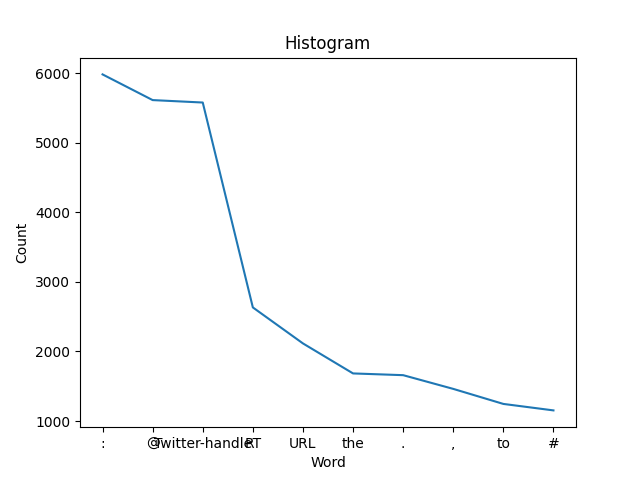
\includegraphics[width=1\textwidth]{../../stats/top_unique_words.png}


	
	
	
\end{document}